\documentclass[11pt]{article}
\usepackage{amssymb}
\usepackage{amsthm}
\usepackage{enumitem}
\usepackage{physics,amsmath}
\usepackage{bm}
\usepackage{adjustbox}
\usepackage{mathrsfs}
\usepackage{graphicx}
\usepackage{siunitx}
\usepackage[mathscr]{euscript}


\title{\textbf{Solved selected problems of General Relativity - Thomas A. Moore}}
\author{Franco Zacco}
\date{}

\addtolength{\topmargin}{-3cm}
\addtolength{\textheight}{3cm}

\newcommand{\hatr}{\bm{\hat{r}}}
\newcommand{\hatn}{\bm{\hat{n}}}
\newcommand{\hatx}{\bm{\hat{x}}}
\newcommand{\haty}{\bm{\hat{y}}}
\newcommand{\hatz}{\bm{\hat{z}}}
\newcommand{\hatth}{\bm{\hat{\theta}}}
\newcommand{\hatphi}{\bm{\hat{\phi}}}
\newcommand{\hatrho}{\bm{\hat{\rho}}}
\newcommand{\er}{\bm{e}_r}
\newcommand{\etht}{\bm{e}_\theta}

\theoremstyle{definition}
\newtheorem*{solution*}{Solution}
\renewcommand*{\proofname}{Solution}

\begin{document}
\maketitle
\thispagestyle{empty}

\section*{Chapter 12 - Photon Orbits}

\begin{proof}{\textbf{BOX 12.2} - Exercise 12.2.1.}\\
    Equation (12.2) states that
    \begin{align*}
        0 = -\left(1- \frac{2GM}{r}\right)dt^2
        + \left(1- \frac{2GM}{r}\right)^{-1}dr^2 + r^2d\phi^2
    \end{align*}
    Then dividing by $(1-2GM/r)dt^2$ we get that
    \begin{align*}
        0 = -1 + \left(1- \frac{2GM}{r}\right)^{-2}\left(\dv{r}{t}\right)^2
        + r^2\left(1- \frac{2GM}{r}\right)^{-1}\left(\dv{\phi}{t}\right)^2
    \end{align*}
    Finally, replacing equation (12.1) squared we get that
    \begin{align*}
        1 = \left(1- \frac{2GM}{r}\right)^{-2}\left(\dv{r}{t}\right)^2
        + \frac{b^2}{r^2}\left(1- \frac{2GM}{r}\right)
    \end{align*}
\end{proof}
\cleardoublepage
\begin{proof}{\textbf{BOX 12.3} - Exercise 12.3.1.}\\
    The effective potential energy is
    \begin{align*}
        \tilde{V}(r) = \frac{1}{r^2}\left(1 - \frac{2GM}{r}\right)
    \end{align*}
    Then the extremum of $\tilde{V}(r)$ happens at $d\tilde{V}/dr = 0$
    hence we compute the derivative and we equate it to zero as follows
    \begin{align*}
        -\frac{2}{r^3}\left(1 - \frac{2GM}{r}\right)
        + \frac{1}{r^2}\frac{2GM}{r^2} &= 0\\
        -\frac{2}{r^3} + \frac{4GM}{r^4}
        + \frac{2GM}{r^4} &= 0\\
        \frac{6GM}{r} &= 2\\
        r &= 3GM
    \end{align*}
    Finally we compute $\tilde{V}(3GM)$ as shown below
    \begin{align*}
        \tilde{V}(3GM) &= \frac{1}{9(GM)^2}\left(1 - \frac{2GM}{3GM}\right)\\
        &= \frac{1}{9(GM)^2}\frac{1}{3}\\
        &= \frac{1}{27(GM)^2}
    \end{align*}
\end{proof}
\cleardoublepage
\begin{proof}{\textbf{BOX 12.4} - Exercise 12.4.1.}\\
    In flat spacetime we know that
    \begin{align*}
        b &= \frac{l}{e} = \frac{r^2 d\phi/d\tau}{dt/d\tau} = r^2 \dv{\phi}{t}\\
        0 &= -dt^2 + dr^2 +r^2d\phi^2
    \end{align*}
    Then dividing the second equation by $dt^2$ and replacing
    $b^2/r^2 = r^2 (d\phi/dt)^2$ we get that
    \begin{align*}
        0 &= -1 + \left[\dv{r}{t}\right]^2 + \frac{b^2}{r^2}\\
        \frac{1}{b^2} &= \left[\frac{1}{b^2}\dv{r}{t}\right]^2 + \frac{1}{r^2}
    \end{align*}
    Where in the last step we divided by $b^2$.
\end{proof}
\cleardoublepage
\begin{proof}{\textbf{BOX 12.5} - Exercise 12.5.1.}\\
    In the observer's coordinate system the four-vector $\bm{A}$ has components
    \begin{align*}
        A_{obs}^\mu = \begin{bmatrix}
            A_{obs}^t \\ A_{obs}^x \\ A_{obs}^y \\ A_{obs}^z
        \end{bmatrix}
    \end{align*}
    Also, $\bm{o}_x$ in the observer's reference frame is defined as
    \begin{align*}
        (\bm{o}_x)_{obs}^\mu = \begin{bmatrix}
            0 \\ 1 \\ 0 \\ 0
        \end{bmatrix}
    \end{align*}
    Therefore, the inner product between these vectors in the observer's frame
    is
    \begin{align*}
        \bm{o}_x \cdot \bm{A} = \eta_{\mu\nu}(\bm{o}_x)_{obs}^\mu A_{obs}^\nu
        = \eta_{x\nu}(\bm{o}_x)_{obs}^x A_{obs}^\nu
        = \eta_{x\nu}(1) A_{obs}^\nu
        = \eta_{xx} A_{obs}^x
        = A_{obs}^x
    \end{align*}
\end{proof}
\begin{proof}{\textbf{BOX 12.6} - Exercise 12.6.1.}\\
    Let us compute $(\bm{o}_x)^\mu$, we know that
    $\bm{o}_x \cdot \bm{o}_x = \eta_{xx} = 1$ and since we align $\bm{o}_x$
    with $\phi$ Schwarzschild coordinate the rest of the components must be
    zero and hence 
    \begin{align*}
        1 = \bm{o}_x \cdot \bm{o}_x = g_{\mu\nu}(\bm{o}_x)^\mu(\bm{o}_x)^\nu
        = g_{\phi\phi}(\bm{o}_x)^\phi(\bm{o}_x)^\phi
        = r^2\sin\theta^2((\bm{o}_x)^\phi)^2
    \end{align*}
    Therefore
    \begin{align*}
        (\bm{o}_x)^\phi = \frac{1}{r\sin\theta}
    \end{align*}
    In the same way, for $(\bm{o}_y)^\mu$ and $(\bm{o}_z)^\mu$ where we align
    them with $-\theta$ and $r$ respectively, we have that
    \begin{align*}
        1 = \bm{o}_y \cdot \bm{o}_y = g_{\mu\nu}(\bm{o}_y)^\mu(\bm{o}_y)^\nu
        = g_{\theta\theta}(\bm{o}_y)^\theta(\bm{o}_y)^\theta
        = r^2((\bm{o}_y)^\theta)^2
    \end{align*}
    Therefore $(\bm{o}_y)^\theta = 1/r$ but since it's aligned to $-\theta$
    must be that
    $$(\bm{o}_y)^\theta = -\frac{1}{r}$$
    Finally, for $(\bm{o}_z)^\mu$ we have that
    \begin{align*}
        1 = \bm{o}_z \cdot \bm{o}_z = g_{\mu\nu}(\bm{o}_z)^\mu(\bm{o}_z)^\nu
        = g_{rr}(\bm{o}_z)^r(\bm{o}_z)^r
        = \left(1 - \frac{2GM}{r}\right)^{-1}((\bm{o}_z)^r)^2
    \end{align*}
    Hence
    \begin{align*}
        (\bm{o}_z)^r = \sqrt{1 - \frac{2GM}{r}}
    \end{align*}
\end{proof}
\cleardoublepage
\begin{proof}{\textbf{BOX 12.7}}
    We know that the angle $\psi$ an emitted photon's path makes with the
    outward direction is such that
    \begin{align*}
        \sin\psi = \frac{v_{x,obs}}{1} = \frac{p^x_{obs}}{p^t_{obs}}
        = \frac{\bm{o}_x \cdot \bm{p}}{-\bm{o}_t\cdot\bm{p}}
    \end{align*}
    Then from equations 12.10 and 12.12 we have that
    \begin{align*}
        \sin\psi &= \frac{\bm{o}_x \cdot \bm{p}}{-\bm{o}_t\cdot\bm{p}}\\
        &= \frac{g_{\mu\nu}(\bm{o}_x)^\mu p^\nu}{-g_{\mu\nu}(\bm{o}_t)^\mu p^\nu}\\
        &= \frac{r^2(1/r)(Eb/r^2)}
        {(1 - 2GM/r)(1/\sqrt{1 - 2GM/r})(E/(1 - 2GM/r))}\\
        &= \frac{b/r}{1/\sqrt{1 - 2GM/r}}\\
        &= \frac{b}{r}\sqrt{1 - \frac{2GM}{r}}
    \end{align*}
    Finally, the critical angle correspond to when $b = GM\sqrt{27}$ hence
    \begin{align*}
        \sin\psi_c &= \frac{GM\sqrt{27}}{r}\sqrt{1 - \frac{2GM}{r}}
    \end{align*}
\end{proof}
\cleardoublepage
\begin{proof}{\textbf{P12.1}}
    We know that if $b > \sqrt{27}GM$ then a photon coming in from infinity
    will rebound to infinity.\\
    So if $b = 6GM$ we see that $6GM > \sqrt{27}GM \approx 5.19 GM$
    then the photon will not be absorbed by the black hole but it will rebound
    to infinity.
\end{proof}
\begin{proof}{\textbf{P12.2}}
    We saw that if a photon has $b > \sqrt{27}GM$ then will rebound to infinity
    then the cylindrical beam of photons must have at most a radius
    $R = \sqrt{27}GM$, assuming the center of the beam is aligned
    to the center of the object.
\end{proof}
\begin{proof}{\textbf{P12.3}}
    In BOX 12.7 we computed the $\sin\psi$ which is essentially $v_x$ since
    $\sin\psi = v_{x}/1$ hence
    \begin{align*}
        v_x = \frac{b}{r}\sqrt{1 - \frac{2GM}{r}}
        = \sqrt{\frac{b^2}{r^2}\bigg(1 - \frac{2GM}{r}\bigg)}
    \end{align*}
    In the same way, we compute $v_z$ as follows
    \begin{align*}
        v_z &= \frac{\bm{o}_z \cdot \bm{p}}{-\bm{o}_t\cdot\bm{p}}\\
        &= \frac{g_{\mu\nu}(\bm{o}_z)^\mu p^\nu}{-g_{\mu\nu}(\bm{o}_t)^\mu p^\nu}\\
        &= \frac{(1 - 2GM/r)^{-1}\sqrt{1 - 2GM/r}E\sqrt{1 - b^2/r^2(1- 2GM/r)}}
        {(1 - 2GM/r)(1/\sqrt{1 - 2GM/r})(E/(1 - 2GM/r))}\\
        &= \frac{(1 - 2GM/r)E\sqrt{1 - b^2/r^2(1- 2GM/r)}}
        {(1 - 2GM/r)^2(E/(1 - 2GM/r))}\\
        &= \sqrt{1 - \frac{b^2}{r^2}\bigg(1- \frac{2GM}{r}\bigg)}
    \end{align*}
    Therefore the speed the speed of light moving in the equatorial plane as
    measured by the observer is
    \begin{align*}
        v &= \sqrt{v_x^2 + v_z^2}
        = \sqrt{\frac{b^2}{r^2}\bigg(1 - \frac{2GM}{r}\bigg) + 1 - \frac{b^2}{r^2}\bigg(1- \frac{2GM}{r}\bigg)}
        = 1
    \end{align*}
\end{proof}
\cleardoublepage
\begin{proof}{\textbf{P12.4}}
\begin{itemize}
    \item [\textbf{a.}] When an observer is at rest at $r = 6GM$ the 
    critical angle is given by 
    \begin{align*}
        \psi_c &= \arcsin(\frac{\sqrt{27}GM}{6GM}\sqrt{1 - \frac{2GM}{6GM}})
        = \arcsin(\frac{\sqrt{2}}{2}) = \frac{3\pi}{4} = 135^\circ
    \end{align*}
    Then any light emited beyond $135^\circ$ will be captured by the blackhole
    implying that the blackhole occupy a region between the angles $135^\circ$ and
    $225^\circ$ (measured from the outward direction) or a region of $45^\circ$
    around the inward direction.
    \item [\textbf{b.}]
    \begin{itemize}
        \item When $r = 2.5GM$ then $\psi_c = 68.36^\circ$
        \begin{center}
            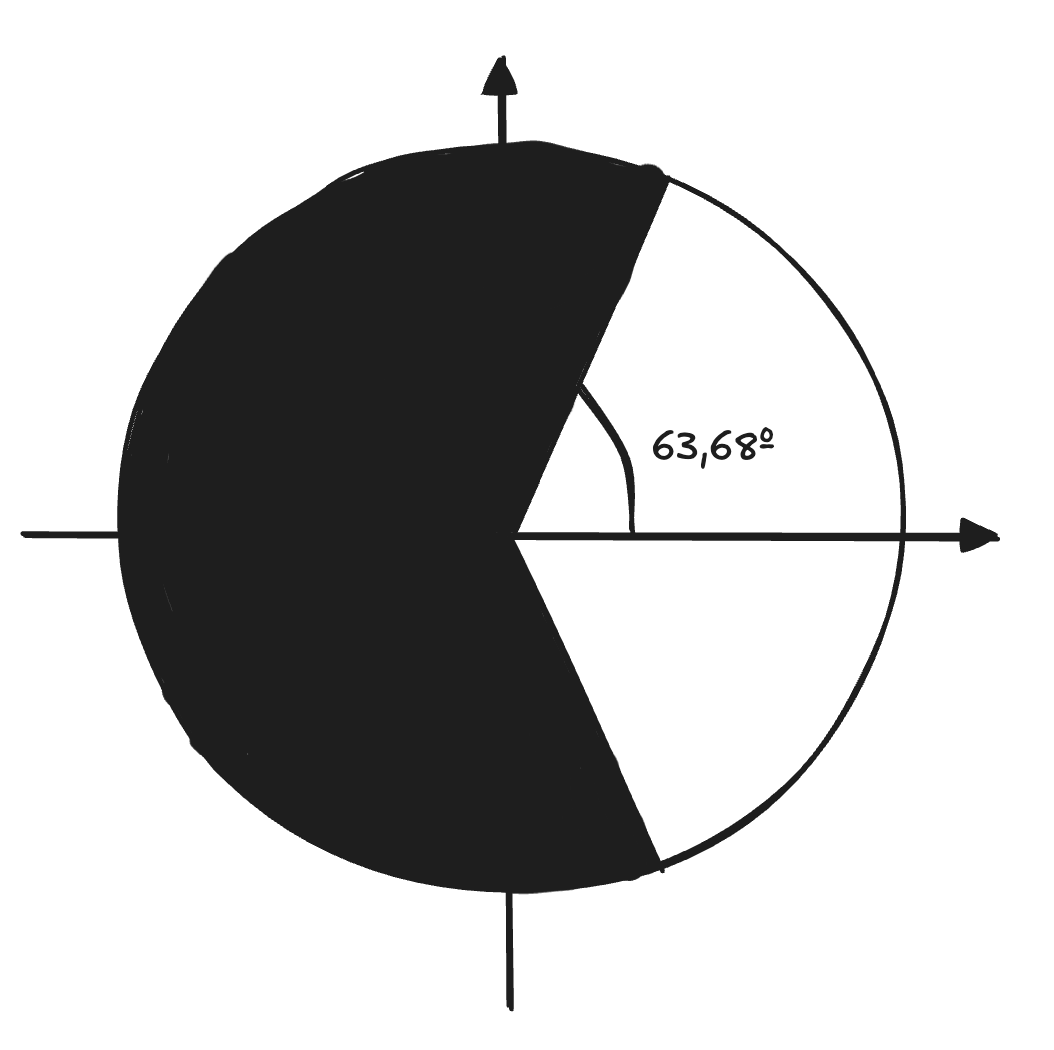
\includegraphics[scale=0.3]{ch12-p12.4-a.png}
        \end{center}
        \item When $r = 3GM$ then $\psi_c = 90^\circ$
        \begin{center}
            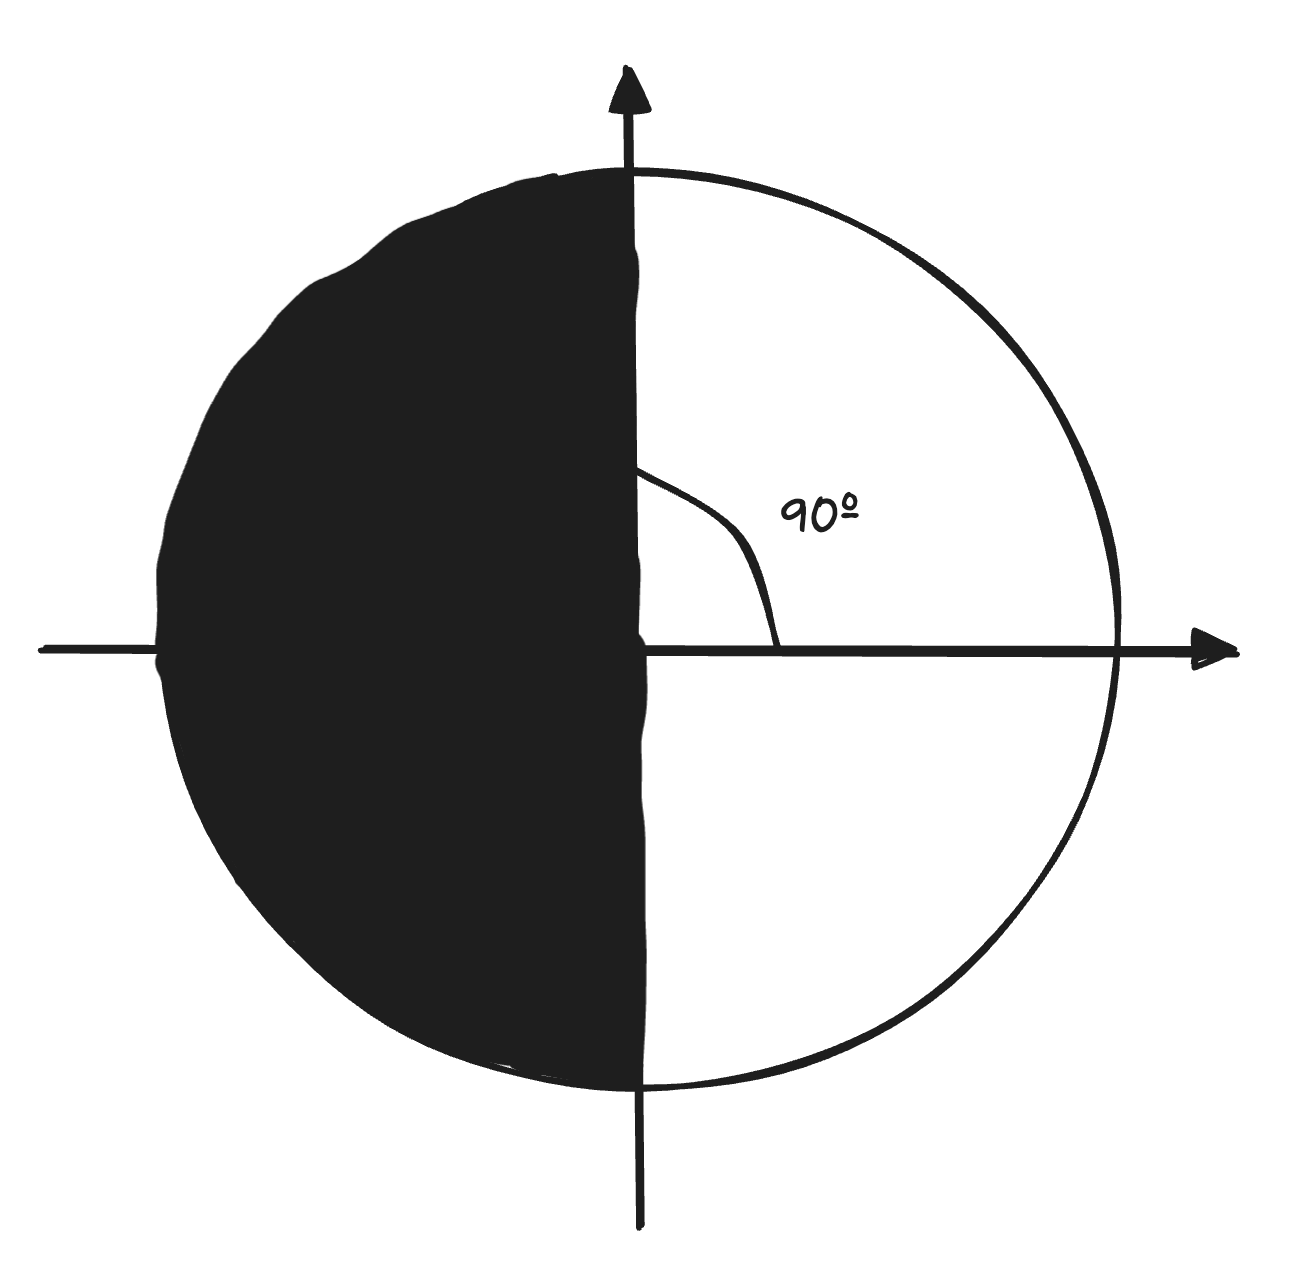
\includegraphics[scale=0.3]{ch12-p12.4-b.png}
        \end{center}
\cleardoublepage
        \item When $r = 4GM$ then $\psi_c = 66.72^\circ = 113.28^\circ$
        \begin{center}
            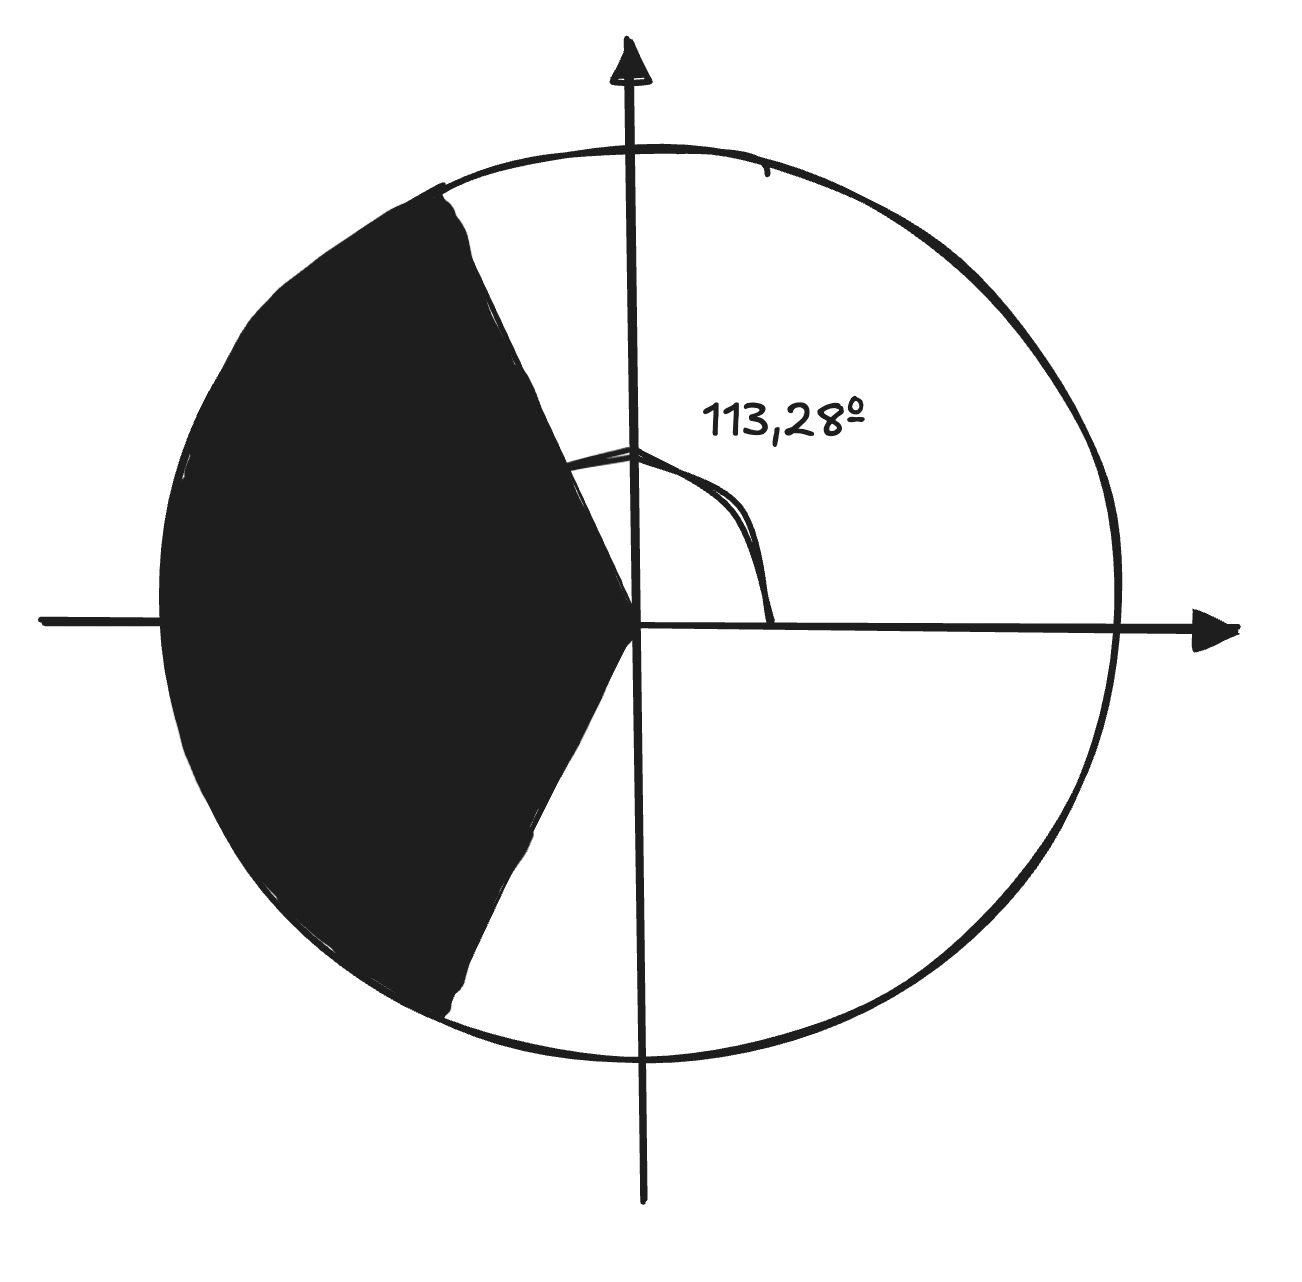
\includegraphics[scale=0.3]{ch12-p12.4-c.png}
        \end{center}
        \item When $r = 5GM$ then $\psi_c = 53.61^\circ = 126.39^\circ$
        \begin{center}
            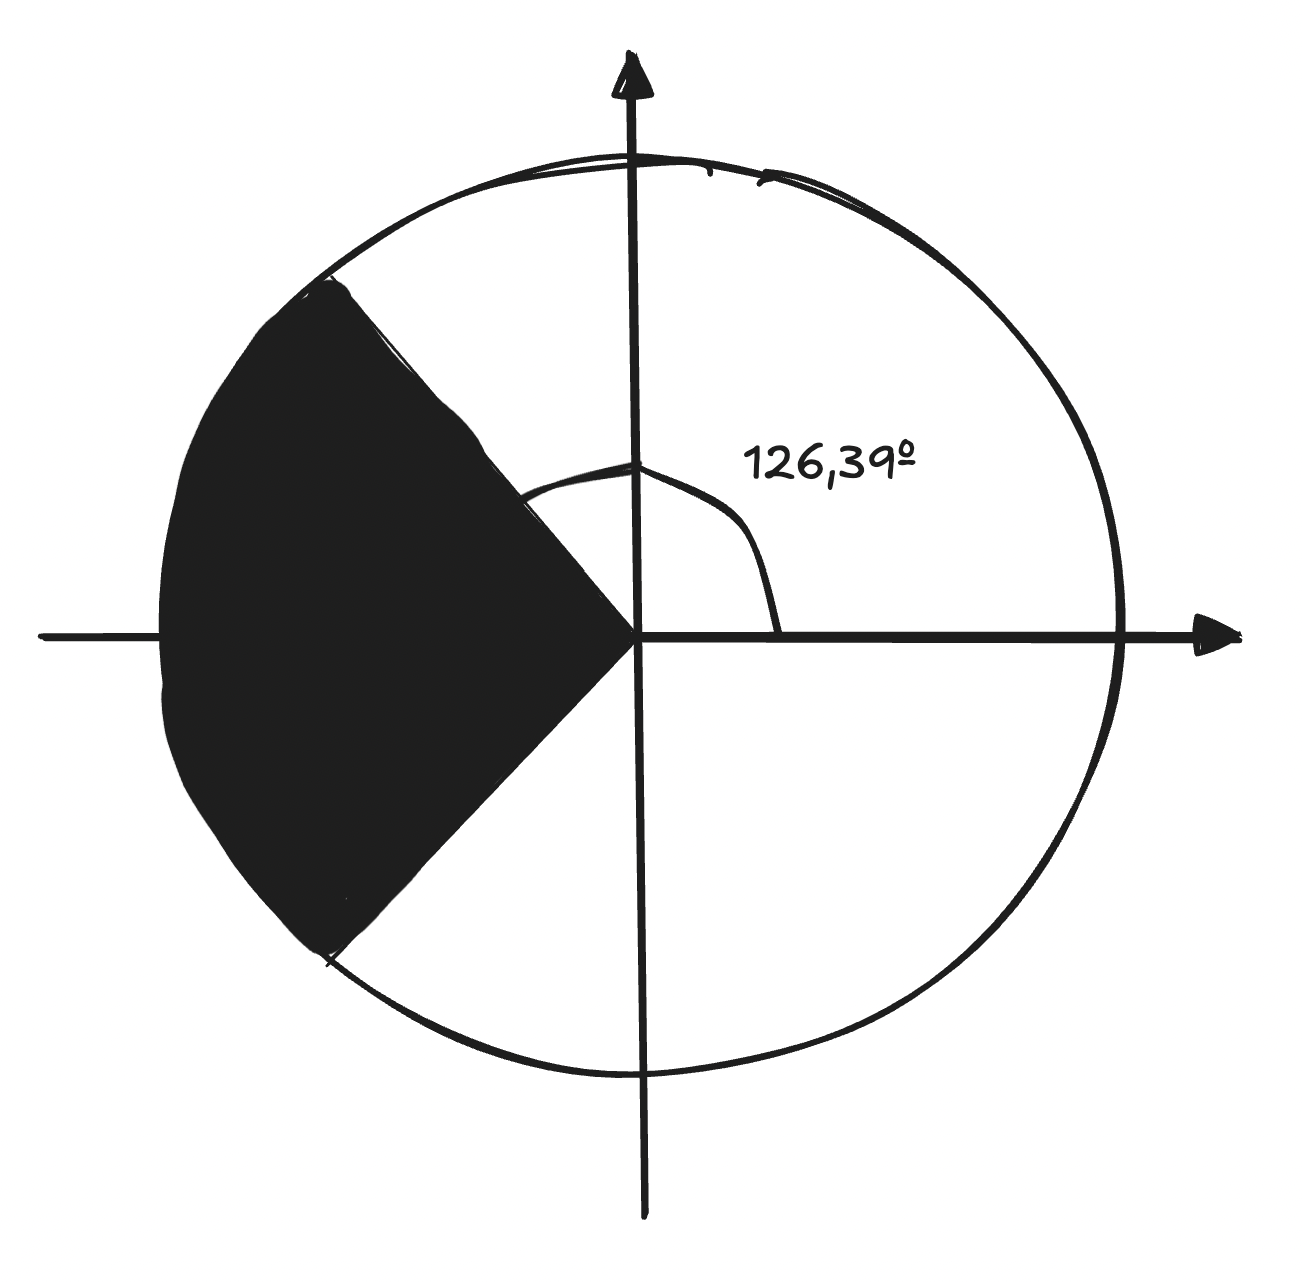
\includegraphics[scale=0.3]{ch12-p12.4-d.png}
        \end{center}
    \end{itemize}
\end{itemize}
\end{proof}
\cleardoublepage
\begin{proof}{\textbf{P12.5}}
    Equation 9.12 states that
    \begin{align*}
        \frac{\lambda_R}{\lambda_E}
        = \frac{\sqrt{1 - 2GM/r_R}}{\sqrt{1 - 2GM/r_E}}
    \end{align*}
    If we consider that $E = h/\lambda$ for a photon, equation 12.15 for
    an observer at $r_R$ becomes
    \begin{align*}
        E_{obs} = \frac{h}{\lambda_R} = \frac{E}{\sqrt{1 - 2GM/r_R}}
    \end{align*}
    And for an observer at $r_E$ we have that
    \begin{align*}
        \frac{h}{\lambda_E} = \frac{E}{\sqrt{1 - 2GM/r_E}}
    \end{align*}
    Hence 
    \begin{align*}
        \frac{h/\lambda_E}{h/\lambda_R}
        &= \frac{E/\sqrt{1 - 2GM/r_E}}{E/\sqrt{1 - 2GM/r_R}}\\
        \frac{\lambda_R}{\lambda_E}
        &= \frac{\sqrt{1 - 2GM/r_R}}{\sqrt{1 - 2GM/r_E}}
    \end{align*}
    Therefore equation 12.15 is consistent with equation 9.12.
\end{proof}
\cleardoublepage
\begin{proof}{\textbf{P12.6}}
\begin{itemize}
    \item [\textbf{a.}] From equation (12.5) we get that
    \begin{align*}
        \frac{1}{b^2} = \bigg[\frac{1}{b}\dv{r}{t}\bigg]^2 + \frac{1}{r^2}
    \end{align*}
    And from equation (12.19) we get that
    \begin{align*}
        b = r^2\dv{\phi}{t} \quad\text{ or }\quad \dv{\phi}{t} = \frac{b}{r^2}
    \end{align*}
    Also, we can combine them as follows
    \begin{align*}
        \bigg[\frac{1}{b}\dv{r}{t}\bigg]^2 &= \frac{1}{b^2} - \frac{1}{r^2}\\
        \bigg[\dv{r}{t}\bigg]^2 &= b^2\bigg(\frac{1}{b^2} - \frac{1}{r^2}\bigg)\\
        \dv{r}{t} &= \pm \sqrt{1 - \frac{b^2}{r^2}}
    \end{align*}
    \item [\textbf{b.}] Let us divide the equations as follows
    \begin{align*}
        \frac{d\phi/dt}{dr/dt} &= \frac{b/r^2}{\sqrt{1 - \frac{b^2}{r^2}}}\\
        \dv{\phi}{r} &= \frac{b}{r^2\sqrt{1 - \frac{b^2}{r^2}}}
    \end{align*}
    Now, integrating leaves us with 
    \begin{align*}
        \int d\phi &= \int \frac{b}{r^2\sqrt{1 - \frac{b^2}{r^2}}}~dr\\
        \phi &= \arccot(\frac{b}{\sqrt{r^2 - b^2}}) + \alpha\\
        \cos(\phi) &= \cos(\arccot(\frac{b}{\sqrt{r^2 - b^2}})) + \alpha\\
        \cos(\phi)
        &= \frac{b/\sqrt{r^2 - b^2}}{\sqrt{1 + (b^2/(r^2 - b^2))}} + \alpha\\
        \cos(\phi)
        &= \frac{b/\sqrt{r^2 - b^2}}{\sqrt{(b^2/(r^2 - b^2))(1 + (r^2 - b^2)/b^2)}} + \alpha\\
        \cos(\phi) &= \frac{1}{\sqrt{1 + (r^2 - b^2)/b^2}} + \alpha\\
        \cos(\phi) &= \frac{1}{\sqrt{1 + r^2/b^2 - 1}} + \alpha\\
        \cos(\phi) &= \frac{b}{r} + \alpha\\
        \phi &= \arccos(\frac{b}{r}) + \alpha
    \end{align*}
    \item [\textbf{c.}] Let $b$ be the smallest distance between the line and
    the origin.

    From the equation we derived in part \textbf{b.} we have that
    \begin{align*}
        \phi - \alpha &= \arccos(\frac{b}{r})\\
        r\cos(\phi - \alpha) &= b\\
        r(\cos\phi\cos\alpha + \sin\phi\sin\alpha) &= b\\
        x\cos\alpha + y\sin\alpha &= b
    \end{align*}
    We used that $x = r\cos\phi$ and $y = r\sin\phi$. 
    Therefore we arrived at the normal equation of a line in rectangular
    coordinates.
\end{itemize}
\end{proof}
\cleardoublepage
\begin{proof}{\textbf{P12.7}}
\begin{itemize}
    \item [\textbf{a.}] Since the observer is falling from rest then $e = 1$
    hence
    \begin{align*}
        \bigg(1 - \frac{2GM}{r}\bigg)\dv{t}{\tau} &= 1\\
        \dv{t}{\tau} &= \bigg(1 - \frac{2GM}{r}\bigg)^{-1}
    \end{align*}
    Also, $l = 0$ since it's falling radially, so $d\phi/d\tau = 0$ so the
    equation of motion becomes
    \begin{align*}
        \frac{1}{2}\bigg(\dv{r}{\tau}\bigg)^{2} - \frac{GM}{r} &= 0\\
        \dv{r}{\tau} &= \pm\sqrt{\frac{2GM}{r}}
    \end{align*}
    Finally, if we assume this to happen on the equatorial plane must be that
    $d\theta/d\tau = 0$.
    \item [\textbf{b.}] Let us compute $\bm{o}_x \cdot \bm{o}_t$ knowing that
    $\bm{o}_x$ is aligned to $\phi$ as follows
    \begin{align*}
        0 = \bm{o}_x \cdot \bm{o}_t
        = g_{\mu\nu} (\bm{o}_x)^\mu(\bm{o}_t)^\nu
        = g_{tt} (\bm{o}_x)^t(\bm{o}_t)^t
        + g_{\phi\phi} (\bm{o}_x)^\phi(\bm{o}_t)^\phi
    \end{align*}
    Since $(\bm{o}_t)^\phi = 0$ then must be that $(\bm{o}_x)^t = 0$.
    Also, since $\bm{o}_x$ has no components in the $r$ and $\theta$ direction
    then computing $\bm{o}_x \cdot \bm{o}_x$ gives us
    \begin{align*}
        1 = \bm{o}_x \cdot \bm{o}_x
        = g_{\mu\nu} (\bm{o}_x)^\mu(\bm{o}_x)^\nu
        = g_{\phi\phi} (\bm{o}_x)^\phi(\bm{o}_x)^\phi
        = r^2\sin^2\theta ((\bm{o}_x)^\phi)^2
    \end{align*}
    So as in equation (12.10), $\bm{o}_x$ is given by
    \begin{align*}
        (\bm{o}_x)^\mu = \begin{bmatrix}
            0\\ 0  \\ 0 \\ \frac{1}{r\sin\theta}
        \end{bmatrix}
    \end{align*}
    Now, let us compute $\bm{o}_y \cdot \bm{o}_t$ so in the same way, we have
    that
    \begin{align*}
        0 = \bm{o}_y \cdot \bm{o}_t
        = g_{\mu\nu} (\bm{o}_y)^\mu(\bm{o}_t)^\nu
        = g_{tt} (\bm{o}_y)^t(\bm{o}_t)^t
        + g_{\phi\phi} (\bm{o}_y)^\theta(\bm{o}_t)^\theta
    \end{align*}
    Which implies that $(\bm{o}_y)^t = 0$ since $(\bm{o}_t)^\theta = 0$
    and hence $(\bm{o}_y)^\mu$ is 
    \begin{align*}
        (\bm{o}_y)^\mu = \begin{bmatrix}
            0\\ 0  \\ -\frac{1}{r} \\ 0
        \end{bmatrix}
    \end{align*}
    Where we used that $1 = r^2 ((\bm{o}_y)^\theta)^2$.

    Finally, let us compute $\bm{o}_z \cdot \bm{o}_t$ then we have that
    \begin{align*}
        0 = \bm{o}_z \cdot \bm{o}_t
        = g_{\mu\nu} (\bm{o}_z)^\mu(\bm{o}_t)^\nu
        = g_{tt} (\bm{o}_z)^t(\bm{o}_t)^t
        + g_{rr} (\bm{o}_z)^r(\bm{o}_t)^r
    \end{align*}
    Then 
    \begin{align*}
        0 &= -\bigg(1 - \frac{2GM}{r}\bigg) (\bm{o}_z)^t \bigg(1 - \frac{2GM}{r}\bigg)^{-1}
        - \bigg(1 - \frac{2GM}{r}\bigg)^{-1} (\bm{o}_z)^r \sqrt{\frac{2GM}{r}}\\
        (\bm{o}_z)^t &=
        - \bigg(1 - \frac{2GM}{r}\bigg)^{-1}\sqrt{\frac{2GM}{r}}(\bm{o}_z)^r
    \end{align*}
    But also if we compute $\bm{o}_z \cdot \bm{o}_z$ we have that
    \begin{align*}
        \bm{o}_z \cdot \bm{o}_z &= 1\\
        g_{\mu\nu} (\bm{o}_z)^\mu(\bm{o}_z)^\nu &= 1\\
        g_{tt} ((\bm{o}_z)^t)^2 + g_{rr} ((\bm{o}_z)^r)^2 &= 1\\
        -\bigg(1 - \frac{2GM}{r}\bigg)((\bm{o}_z)^t)^2
        + \bigg(1 - \frac{2GM}{r}\bigg)^{-1} ((\bm{o}_z)^r)^2 &= 1\\
        -\bigg(1 - \frac{2GM}{r}\bigg)^{-1}\frac{2GM}{r}((\bm{o}_z)^r)^2
        + \bigg(1 - \frac{2GM}{r}\bigg)^{-1} ((\bm{o}_z)^r)^2 &= 1\\
        \bigg(1 -\frac{2GM}{r}\bigg)
        \bigg(1 - \frac{2GM}{r}\bigg)^{-1} ((\bm{o}_z)^r)^2 &= 1\\
        (\bm{o}_z)^r &= 1
    \end{align*}
    Where we replaced the value fore $(\bm{o}_z)^t$. Therefore $(\bm{o}_z)^\mu$
    is
    \begin{align*}
        (\bm{o}_z)^\mu = \begin{bmatrix}
            \frac{-\sqrt{2GM/r}}{1 - 2GM/r}\\
            1 \\ 0 \\ 0
        \end{bmatrix}
    \end{align*}
    \item [\textbf{c.}] Let us compute the critical angle using equation
    (12.13) as follows
    \begin{align*}
        \sin\psi &= \frac{\bm{o}_x\cdot \bm{p}}{-\bm{o}_t\cdot \bm{p}}\\
        &= \frac{g_{\mu\nu}(\bm{o}_x)^\mu (\bm{p})^\nu}
        {-g_{\mu\nu}(\bm{o}_t)^\mu (\bm{p})^\nu}\\
        &= \frac{r^2\frac{1}{r}\frac{Eb}{r^2}}
        {E(1 - \frac{2GM}{r})^{-1} \pm (1 - \frac{2GM}{r})^{-1}
        \sqrt{\frac{2GM}{r}}E\sqrt{1 - \frac{b^2}{r^2}(1 - \frac{2GM}{r})}}\\
        &= \frac{\frac{b}{r}(1 - \frac{2GM}{r})}
        {1 \pm \sqrt{\frac{2GM}{r}}\sqrt{1 - \frac{b^2}{r^2}(1 - \frac{2GM}{r})}}
    \end{align*}
    Then setting $b = \sqrt{27}GM$ to get the critical angle we have that
    \begin{align*}
        \sin\psi_c
        &= \frac{\frac{\sqrt{27}GM}{r}(1 - \frac{2GM}{r})}
        {1 \pm \sqrt{\frac{2GM}{r}}\sqrt{1 - \frac{27(GM)^2}{r^2}(1 - \frac{2GM}{r})}}\\
    \end{align*}
    Where the plus sign in the denominator implies an outgoing photon and the
    minus sign implies an ingoing photon. We see that for $r > 3GM$ the photon
    must be outgoing and for $r < 3GM$ the photon is incoming.
    Then if $r = 4GM$ we have that
    \begin{align*}
        \sin\psi_c
        &= \frac{\frac{\sqrt{27}}{4}(1 - \frac{1}{2})}
        {1 + \sqrt{\frac{1}{2}}\sqrt{1 - \frac{27}{16}(1 - \frac{1}{2})}}
        = 0.5076
    \end{align*}
    Hence $\psi_c = 30.506^\circ = 149.506 ^\circ$
    \begin{center}
        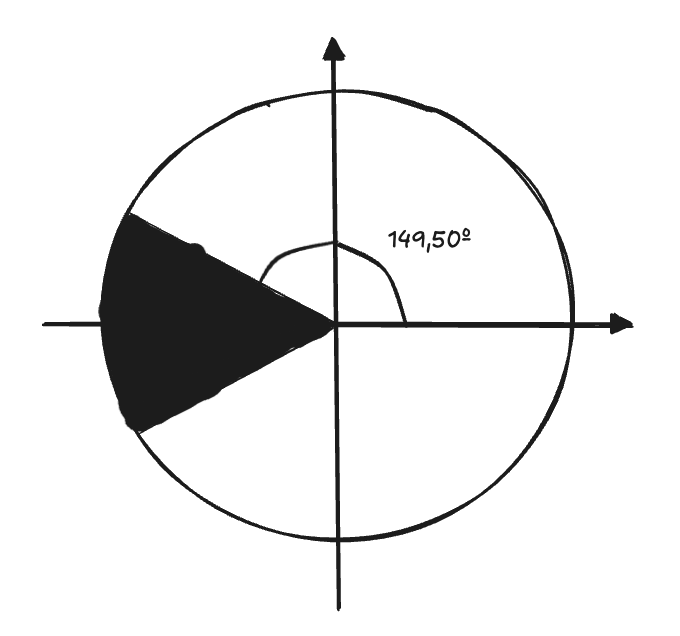
\includegraphics[scale=0.3]{ch12-p12.7-i.png}
    \end{center}
    If $r = 3GM$ then $\psi_c = 35.264^\circ = 144.736^\circ$
    \begin{center}
        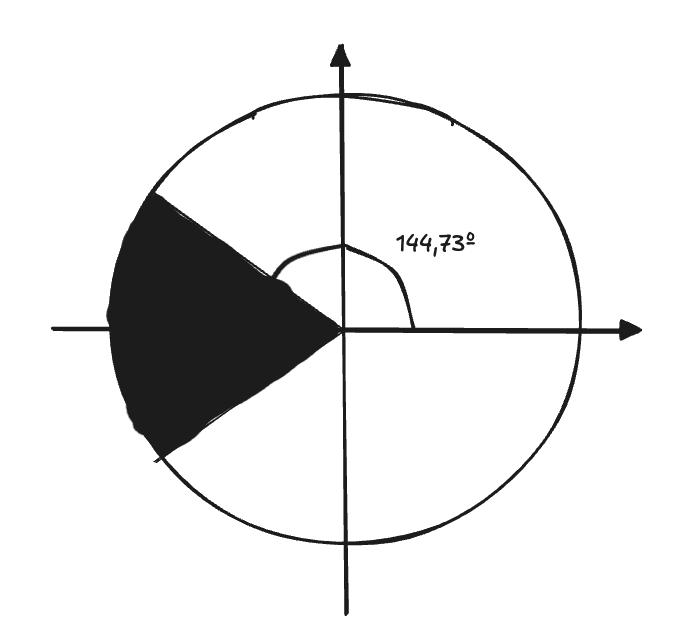
\includegraphics[scale=0.3]{ch12-p12.7-ii.png}
    \end{center}
    If $r = 2GM$ when using the minus sign in the equation we get a 0/0
    indeterminate form so we use l'Hopital rule to compute the limit as follows
    \begin{align*}
        \sin\psi_c
        &= \lim_{r\to 2GM}
        \frac{\frac{\sqrt{27}GM}{r}(1 - \frac{2GM}{r})}
        {1 - \sqrt{\frac{2GM}{r}}\sqrt{1 - \frac{27(GM)^2}{r^2}(1 - \frac{2GM}{r})}}\\
        &= \lim_{r\to 2GM}
        \frac{\frac{3\sqrt{3GM}}{r^3}(4GM - r)}
        {\frac{\sqrt{GM/r}(216(GM)^3 - 81(GM)^2r + r^3)}{\sqrt{2}r^4\sqrt{(r-3GM)^2(6GM + r)/r^3}}}\\
        &= \frac{12\sqrt{3}}{31} 
    \end{align*}
    then $\psi_c = 42.103^\circ = 138.897^\circ$
    \begin{center}
        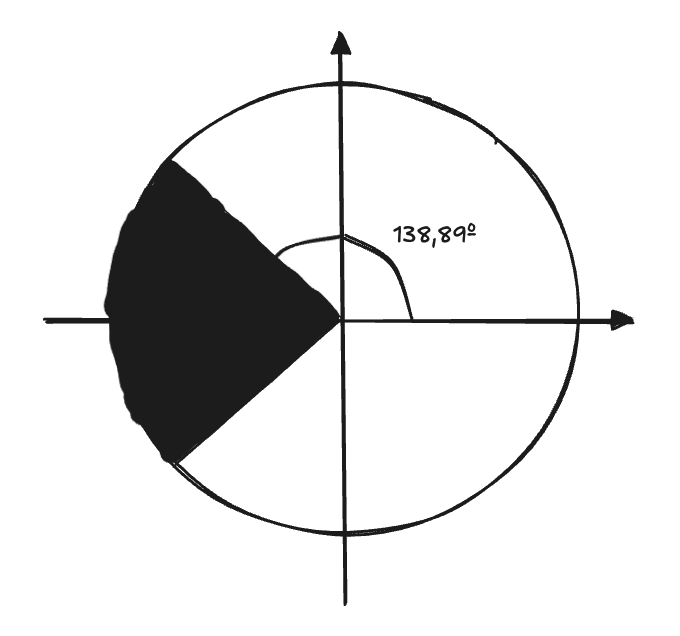
\includegraphics[scale=0.3]{ch12-p12.7-iii.png}
    \end{center}
    Finally for $r = GM$ we have that $\psi_c = 53.27^\circ = 126.72^\circ$
    \begin{center}
        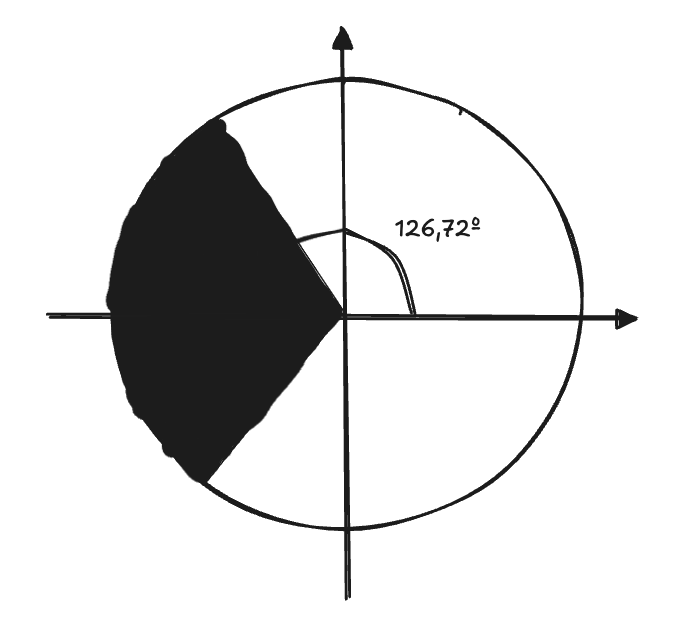
\includegraphics[scale=0.3]{ch12-p12.7-iv.png}
    \end{center}
    \item[\textbf{d.}]
    The incoming photon's energy a falling observer measures is
    \begin{align*}
        E_{obs} &= - \bm{o}_t \cdot \bm{p}\\
        &= E\bigg(1 - \frac{2GM}{r}\bigg)^{-1} - \bigg(1 - \frac{2GM}{r}\bigg)^{-1}
        \sqrt{\frac{2GM}{r}}E\sqrt{1 - \frac{b^2}{r^2}\bigg(1 - \frac{2GM}{r}\bigg)}\\
        &= E\bigg(1 - \frac{2GM}{r}\bigg)^{-1}
        \bigg(1 - \sqrt{\frac{2GM}{r}}
        \sqrt{1 - \frac{b^2}{r^2}\bigg(1 - \frac{2GM}{r}\bigg)}\bigg)
    \end{align*}
    But since it's falling radially then $b = 0$ so
    \begin{align*}
        E_{obs} &= E\bigg(1 - \frac{2GM}{r}\bigg)^{-1}
        \bigg(1 - \sqrt{\frac{2GM}{r}}\bigg)
    \end{align*}
    Then we see that $E_{obs} < E$ so the observer receives signals red-shifted.

    Finally, the fractional change in wavelength is given by
    \begin{align*}
        \frac{h/\lambda_E}{h/\lambda_R}
        &= \frac{E/\sqrt{1 - \frac{2GM}{r_E}}}{E\bigg(1 - \frac{2GM}{r_R}\bigg)^{-1}
        \bigg(1 - \sqrt{\frac{2GM}{r_R}}\bigg)}\\
        \frac{\lambda_R}{\lambda_E}
        &= \frac{\bigg(1 - \frac{2GM}{r_R}\bigg)}{\sqrt{1 - \frac{2GM}{r_E}}
        \bigg(1 - \sqrt{\frac{2GM}{r_R}}\bigg)}
    \end{align*}
    But since $r_E = \infty$ i.e. the signal is coming from infinity
    we can write that
    \begin{align*}
        \frac{\lambda_R}{\lambda_E}
        &= \frac{\bigg(1 - \frac{2GM}{r_R}\bigg)}
        {\bigg(1 - \sqrt{\frac{2GM}{r_R}}\bigg)}
    \end{align*}
\end{itemize}
\end{proof}
\cleardoublepage
\begin{proof}{\textbf{P12.8}}
    In the falling observer's frame the velocity components of the object in
    circular orbit are $u^t_{obs} = -\bm{o}_t\cdot\bm{u}$ and 
    $u^\mu_{obs} = \bm{o}_\mu\cdot\bm{u}$ for the spatial components.
    Then
    \begin{align*}
        u^t_{obs} &= -\bm{o}_t\cdot\bm{u}\\
        &= -g_{\mu\nu}(\bm{o}_t)^\mu (\bm{u})^\nu\\
        &= -(g_{tt}(\bm{o}_t)^tu^t + g_{rr}(\bm{o}_t)^ru^r)\\
        &= \bigg(1- \frac{2GM}{r}\bigg)\bigg(1- \frac{2GM}{r}\bigg)^{-1}u^t
        + \bigg(1- \frac{2GM}{r}\bigg)^{-1}\sqrt{\frac{2GM}{r}} u^r\\
        &= u^t
    \end{align*}
    Where we used that $u^r = 0$ for an object in a circular orbit.
    Also, we see that
    \begin{align*}
        u^x_{obs} &= \bm{o}_x\cdot\bm{u}
        = g_{\mu\nu}(\bm{o}_x)^\mu (\bm{u})^\nu
        = g_{\phi\phi}(\bm{o}_x)^\phi (\bm{u})^\phi
        = r^2\frac{1}{r}u^{\phi}
        = ru^{\phi}\\
        u^z_{obs} &= \bm{o}_z\cdot\bm{u}
        = g_{\mu\nu}(\bm{o}_z)^\mu (\bm{u})^\nu
        = g_{tt}(\bm{o}_z)^t (\bm{u})^t + g_{rr}(\bm{o}_z)^r (\bm{u})^r
        = \sqrt{\frac{2GM}{r}}u^t
    \end{align*}

    On the other hand, we know that for an object in circular orbit at
    $r =6GM$ we have that $l = \sqrt{12}GM$ and $e = \sqrt{8/9}$ hence
    \begin{align*}
        u^t_{obs} &= u^t = \dv{t}{\tau} = e\bigg(1- \frac{2GM}{r}\bigg)^{-1}
        = \sqrt{\frac{8}{9}}\bigg(\frac{2}{3}\bigg)^{-1}
        = \sqrt{2}\\
        u^x_{obs} &= ru^\phi = r\dv{\phi}{\tau} = \frac{l}{r}
        = \frac{\sqrt{12}GM}{6GM}
        = \frac{\sqrt{3}}{3}\\
        u^z_{obs} &= \sqrt{\frac{2GM}{r}}u^t
        = e\sqrt{\frac{2GM}{r}}\bigg(1- \frac{2GM}{r}\bigg)^{-1}
        = \sqrt{\frac{8}{9}}\sqrt{\frac{1}{3}}\bigg(\frac{2}{3}\bigg)^{-1}
        = \frac{\sqrt{6}}{3}
    \end{align*}
    Finally, the speed in the observer's frame is
    \begin{align*}
        v &= \sqrt{v_x^2 + v_z^2}\\
        &= \sqrt{
            \left(\frac{u_{obs}^x}{u_{obs}^t}\right)^2
            + \left(\frac{u_{obs}^z}{u_{obs}^t}\right)^2
        }\\
        &= \sqrt{
            \bigg(\frac{\sqrt{3}}{3\sqrt{2}}\bigg)^2
            + \bigg(\frac{\sqrt{6}}{3\sqrt{2}}\bigg)^2
        }\\
        &= \sqrt{\frac{1}{6} + \frac{1}{3}}\\
        &= \frac{\sqrt{2}}{2}
    \end{align*}
\end{proof}
\cleardoublepage
\begin{proof}{\textbf{P12.9}}
    For an observer in a circular orbit of radius $r$ we have that
    \begin{align*}
        \dv{t}{\tau} &= e\bigg(1 - \frac{2GM}{r}\bigg)^{-1}
        \quad \dv{r}{\tau} = 0
        \quad \dv{\theta}{\tau} = 0
        \quad \dv{\phi}{\tau} = \frac{l}{r^2}
    \end{align*}
    But also using the equation for the radius of circular orbits we get that
    \begin{align*}
        l = \frac{\sqrt{GM}r}{\sqrt{r - 3GM}}
    \end{align*}
    Also, we know that the equation of $e$ for a circular orbit
    ($\dv{r}{\tau} = 0$) becomes
    \begin{align*}
        e^2 &= -\frac{2GM}{r} + \frac{l^2}{r^2} - \frac{2GMl^2}{r^3} + 1\\
        e &= \sqrt{-\frac{2GM}{r} + \frac{GM}{r - 3GM}
        - \frac{2(GM)^2}{r(r - 3GM)} + 1}\\
        e &= \sqrt{\frac{-2GM(r - 3GM) + GMr - 2(GM)^2 + r^2 - 3GMr}{r(r - 3GM)}}\\
        e &= \sqrt{\frac{4(GM)^2 - 4GMr + r^2}{r(r - 3GM)}}\\
        e &= (r - 2GM)\sqrt{\frac{1}{r(r - 3GM)}}
    \end{align*}
    Hence
    \begin{align*}
        (\bm{o}_t)^\mu = \begin{bmatrix}
        \sqrt{\frac{r}{r - 3GM}}\\
        0\\ 0 \\
        \frac{\sqrt{GM}}{r\sqrt{r - 3GM}}
        \end{bmatrix} 
    \end{align*}
    Where we used that
    $(r - 2GM)\sqrt{\frac{1}{r(r - 3GM)}}\bigg(1 - \frac{2GM}{r}\bigg)^{-1}
    =\sqrt{\frac{r}{r - 3GM}}$.\\
    Now, let us compute $\bm{o}_x\cdot \bm{o}_t$ knowing that $\bm{o}_x$ is
    aligned to $\phi$ as follows 
    \begin{align*}
        0 = \bm{o}_x \cdot \bm{o}_t
        = g_{\mu\nu} (\bm{o}_x)^\mu (\bm{o}_t)^\nu
        = g_{tt} (\bm{o}_x)^t (\bm{o}_t)^t + g_{\phi\phi} (\bm{o}_x)^\phi (\bm{o}_t)^\phi=\\
        = -\bigg(1 - \frac{2GM}{r}\bigg)\sqrt{\frac{r}{r - 3GM}} (\bm{o}_x)^t
        + r^2 \frac{\sqrt{GM}}{r\sqrt{r - 3GM}} (\bm{o}_x)^\phi
    \end{align*}
    Then
    \begin{align*}
        \bigg(1 - \frac{2GM}{r}\bigg)\sqrt{\frac{r}{r - 3GM}} (\bm{o}_x)^t
        &= \frac{r\sqrt{GM}}{r\sqrt{r - 3GM}} (\bm{o}_x)^\phi\\
        (\bm{o}_x)^t
        &= \bigg(1 - \frac{2GM}{r}\bigg)^{-1}\sqrt{\frac{r - 3GM}{r}}
        \frac{r\sqrt{GM}}{\sqrt{r - 3GM}} (\bm{o}_x)^\phi\\
        (\bm{o}_x)^t &= \sqrt{GMr}\bigg(1 - \frac{2GM}{r}\bigg)^{-1}(\bm{o}_x)^\phi\\
    \end{align*}
    Also, for $\bm{o}_x \cdot \bm{o}_x$ we have that
    \begin{align*}
        1 &= \bm{o}_x \cdot \bm{o}_x
        = g_{\mu\nu} (\bm{o}_x)^\mu (\bm{o}_x)^\nu
        = g_{tt} ((\bm{o}_x)^t)^2 + g_{\phi\phi} ((\bm{o}_x)^\phi)^2\\
        &= -\bigg(1 - \frac{2GM}{r}\bigg) ((\bm{o}_x)^t)^2
        + r^2 ((\bm{o}_x)^\phi)^2
    \end{align*}
    So replacing $(\bm{o}_x)^t$ we get that
    \begin{align*}
        1 &= -GMr\bigg(1 - \frac{2GM}{r}\bigg)\bigg(1 - \frac{2GM}{r}\bigg)^{-2}
        ((\bm{o}_x)^\phi)^2 + r^2 ((\bm{o}_x)^\phi)^2\\
        1 &= ((\bm{o}_x)^\phi)^2\bigg(r^2-GMr\bigg(1 - \frac{2GM}{r}\bigg)^{-1}\bigg)\\
        1 &= ((\bm{o}_x)^\phi)^2\bigg(r^2-\frac{GMr^2}{r - 2GM}\bigg)\\
        1 &= ((\bm{o}_x)^\phi)^2r^2\bigg(\frac{r - 3GM}{r - 2GM}\bigg)\\
        ((\bm{o}_x)^\phi)^2 &= \frac{1}{r^2}\bigg(\frac{r - 2GM}{r - 3GM}\bigg)\\
        (\bm{o}_x)^\phi &= \frac{1}{r}\sqrt{\frac{r - 2GM}{r - 3GM}}
    \end{align*}
    Then $(\bm{o}_x)^t$ is 
    \begin{align*}
        (\bm{o}_x)^t
        &= \sqrt{GMr}\bigg(1 - \frac{2GM}{r}\bigg)^{-1}
        \frac{1}{r}\sqrt{\frac{r - 2GM}{r - 3GM}}\\
        &= \frac{\sqrt{GMr}}{r - 2GM}\sqrt{\frac{r - 2GM}{r - 3GM}}\\
        &= \sqrt{\frac{GMr}{(r - 2GM)(r - 3GM)}}
    \end{align*}
    Let us compute now $\bm{o}_y\cdot \bm{o}_t$ as follows
    \begin{align*}
        0 = \bm{o}_y \cdot \bm{o}_t
        = g_{\mu\nu} (\bm{o}_y)^\mu (\bm{o}_t)^\nu
        = g_{tt} (\bm{o}_y)^t (\bm{o}_t)^t + g_{\theta\theta} (\bm{o}_y)^\theta (\bm{o}_t)^\theta
    \end{align*}
    Since $(\bm{o}_t)^\theta = 0$ then must be that $(\bm{o}_y)^t = 0$.
    So from $\bm{o}_y\cdot \bm{o}_y$ we get $(\bm{o}_y)^\theta$ as follows
    \begin{align*}
        1 = \bm{o}_y \cdot \bm{o}_y
        = g_{\mu\nu} (\bm{o}_y)^\mu (\bm{o}_y)^\nu
        = g_{\theta\theta} ((\bm{o}_y)^\theta)^2
        = r^2 ((\bm{o}_y)^\theta)^2
    \end{align*}
    Then $(\bm{o}_y)^\theta = -1/r$ since it's aligned to $-\theta$.
    In the same way, for $(\bm{o}_z)^\mu$ we have that $(\bm{o}_z)^t = 0$
    since $(\bm{o}_t)^r = 0$ and hence the only non-zero component is
    \begin{align*}
        1 = \bm{o}_z \cdot \bm{o}_z
        = g_{\mu\nu} (\bm{o}_z)^\mu (\bm{o}_z)^\nu
        = g_{rr} ((\bm{o}_z)^r)^2
        = \bigg(1 - \frac{2GM}{r}\bigg)^{-1}((\bm{o}_z)^r)^2
    \end{align*}
    Then
    \begin{align*}
        (\bm{o}_z)^r = \sqrt{1 - \frac{2GM}{r}}
    \end{align*}
    Therefore the set of orthonormal basis vectors is
    \begin{align*}
        &(\bm{o}_t)^\mu = \begin{bmatrix}
            \sqrt{\frac{r}{r - 3GM}}\\
            0\\ 0 \\
            \frac{\sqrt{GM}}{r\sqrt{r - 3GM}}
        \end{bmatrix}
        \quad (\bm{o}_x)^\mu = \begin{bmatrix}
            \sqrt{\frac{GMr}{(r - 2GM)(r - 3GM)}}\\
            0\\ 0 \\
            \frac{1}{r}\sqrt{\frac{r - 2GM}{r - 3GM}}
        \end{bmatrix}\\
        &(\bm{o}_y)^\mu = \begin{bmatrix}
            0\\ 0\\ -\frac{1}{r} \\ 0
        \end{bmatrix}
        \quad (\bm{o}_z)^\mu = \begin{bmatrix}
            0\\ \sqrt{1 - \frac{2GM}{r}}\\ 0 \\ 0
        \end{bmatrix}
    \end{align*}
    If $r \leq 3GM$ then $l^2$ will be negative hence no circular orbits can
    exist for $r \leq 3GM$.
\end{proof}
\end{document}